% Major arc about 0 and minor arcs on the rest of [-1/2,1/2], drawn for n=100.
% Top row is to scale: y=0.0204. The lower row magnifies the centre by 10.
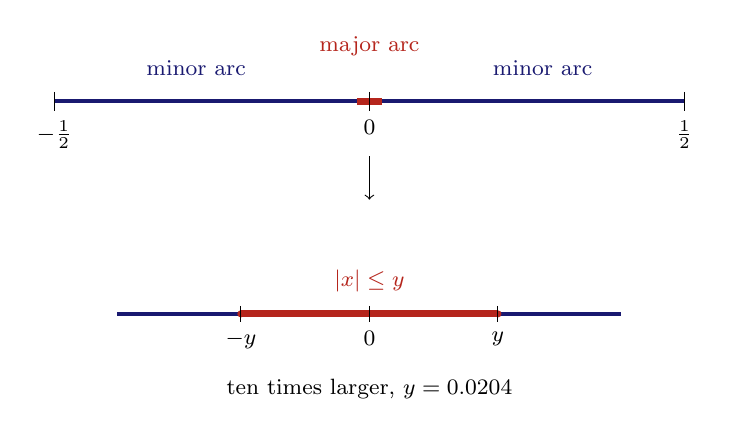
\begin{tikzpicture}[every node/.style={font=\footnotesize}]
  \draw[MidnightBlue,line width=1.5pt] (-4,0)--(-0.163,0);
  \draw[MidnightBlue,line width=1.5pt] (0.163,0)--(4,0);
  \draw[BrickRed,line width=2.4pt] (-0.163,0)--(0.163,0);
  \draw (-4,0.12)--(-4,-0.12) node[below] {$-\frac12$};
  \draw (4,0.12)--(4,-0.12) node[below] {$\frac12$};
  \draw (0,0.12)--(0,-0.12) node[below] {$0$};
  \node[MidnightBlue,above] at (-2.2,0.2) {minor arc};
  \node[MidnightBlue,above] at (2.2,0.2) {minor arc};
  \node[BrickRed,above] at (0,0.45) {major arc};
  \draw[->,black] (0,-0.7)--(0,-1.25);
  \begin{scope}[yshift=-2.7cm]
    \draw[MidnightBlue,line width=1.3pt] (-3.2,0)--(-1.632,0);
    \draw[MidnightBlue,line width=1.3pt] (1.632,0)--(3.2,0);
    \draw[BrickRed,line width=2.6pt] (-1.632,0)--(1.632,0);
    \fill[BrickRed] (-1.632,0) circle (1.3pt);
    \fill[BrickRed] (1.632,0) circle (1.3pt);
    \draw (-1.632,0.1)--(-1.632,-0.1) node[below] {$-y$};
    \draw (1.632,0.1)--(1.632,-0.1) node[below] {$y$};
    \draw (0,0.1)--(0,-0.1) node[below] {$0$};
    \node[BrickRed,above] at (0,0.15) {$|x|\le y$};
    \node[below] at (0,-0.7) {ten times larger, $y=0.0204$};
  \end{scope}
\end{tikzpicture}
